\exercisesection{1}


\begin{enumerate}
\def\labelenumi{\arabic{enumi}.}
\tightlist
\item
  在交换图 (10) 中，假设有序偶 \((u', v')\) 是一个正合序列，且 \(v \circ u = 0\) 。证明
\end{enumerate}

\(\operatorname{Im}(b) \cap \operatorname{Im}(u') = b(\operatorname{Ker}(c \circ v))\) 且 \(\operatorname{Ker}(b) + \operatorname{Ker}(v) = b^{-1}(\operatorname{Im}(u' \circ a)).\)

\begin{enumerate}
\def\labelenumi{\arabic{enumi}.}
\setcounter{enumi}{1}
\tightlist
\item
  考虑交换群的交换图
\end{enumerate}

\pandocbounded{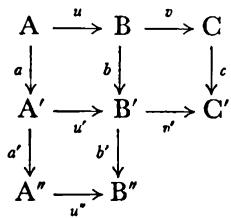
\includegraphics[keepaspectratio]{images/part001_696e1539.jpg}}

假设：(1) \((u, v)\) 与 \((b, b')\) 是正合序列；(2) \(v' \circ u' = 0\) 且 \(a' \circ a = 0\) ；(3) \(c\) 与 \(u'\) 是单射且 \(a'\) 是满射。证明在这些条件下 \(u''\) 是单射。

\begin{enumerate}
\def\labelenumi{\arabic{enumi}.}
\setcounter{enumi}{2}
\tightlist
\item
  考虑交换群的交换图
\end{enumerate}

\pandocbounded{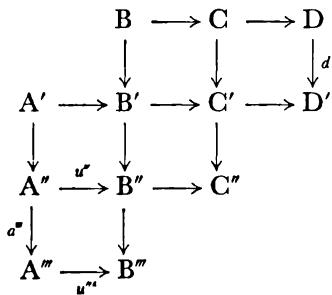
\includegraphics[keepaspectratio]{images/part001_1549be15.jpg}}

其中设各行与各列都正合，d 与 \(u''\) 是单射，\(a''\) 是满射。证明在这些条件下 \(u'''\) 是单射。推广这个结果。

\begin{enumerate}
\def\labelenumi{\arabic{enumi}.}
\setcounter{enumi}{3}
\tightlist
\item
  考虑交换群的交换图
\end{enumerate}

\pandocbounded{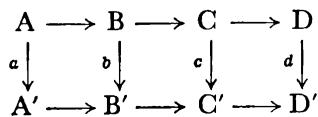
\includegraphics[keepaspectratio]{images/part001_0674edfc.jpg}}

其中设两行都是正合的。

\begin{enumerate}
\def\labelenumi{(\alph{enumi})}
\item
  证明：若 \(a\) 是满射且 \(b\) 与 \(d\) 是单射，则 \(c\) 是单射。
\item
  证明：若 \(d\) 是单射且 \(a\) 与 \(c\) 是满射，则 \(b\) 是满射。
\end{enumerate}

\begin{enumerate}
\def\labelenumi{\arabic{enumi}.}
\setcounter{enumi}{4}
\tightlist
\item
  设给定正合序列 \(A^{\prime} \xrightarrow{u} A \xrightarrow{v} A^{\prime\prime} \to 0\) 与两个满同态 \(B^{\prime} \xrightarrow{a^{\prime}} A^{\prime}, B^{\prime\prime} \xrightarrow{a^{\prime\prime}} A^{\prime\prime}\) ，其中 A, A', A'', B', B'' 是同一个环上的模。证明：若 \(B^{\prime\prime}\) 是投射模，则存在满同态 \(a: B^{\prime} \oplus B^{\prime\prime} \to A\) 使图
\end{enumerate}

\pandocbounded{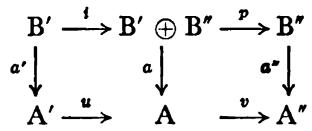
\includegraphics[keepaspectratio]{images/part001_093beead.jpg}}

是交换的（i 与 p 是典范映射）。

\begin{enumerate}
\def\labelenumi{\arabic{enumi}.}
\setcounter{enumi}{5}
\tightlist
\item
  设给定正合序列 \(0 \to A' \xrightarrow{u} A \xrightarrow{v} A''\) 与两个单同态 \(A' \xrightarrow{a'} C', A'' \xrightarrow{a''} C''\) ，其中 \(A, A', A'', C', C''\) 是同一个环上的模。证明：若 \(C'\) 是内射模（《代数学》第二章 §2 习题 11），则存在单同态 \(a: A \to C' \oplus C''\) 使图
\end{enumerate}

\pandocbounded{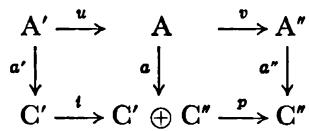
\includegraphics[keepaspectratio]{images/part001_5ee4bea9.jpg}}

是交换的（i 与 p 是典范映射）。

\begin{enumerate}
\def\labelenumi{\arabic{enumi}.}
\setcounter{enumi}{6}
\tightlist
\item
  设 U、V、W 是三个交换群， \(f: \mathrm{U} \to \mathrm{V}\) ， \(g: \mathrm{V} \to \mathrm{W}\) 是同态。
\end{enumerate}

\begin{enumerate}
\def\labelenumi{(\alph{enumi})}
\tightlist
\item
  考虑图
\end{enumerate}

\pandocbounded{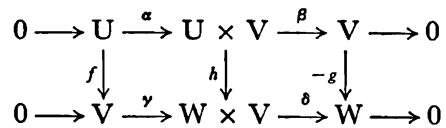
\includegraphics[keepaspectratio]{images/part001_5d67b0a0.jpg}}

其中 \(\alpha(u) = (u, f(u)), \beta(u, v) = v - f(u), \gamma(v) = (g(v), v), \delta(w, v) = w - g(v)\) ， \(h(u, v) = (g(f(u)), v)\) 。证明这个图是交换的且它的各行是正合的。

\begin{enumerate}
\def\labelenumi{(\alph{enumi})}
\setcounter{enumi}{1}
\tightlist
\item
  由 (a) 与第 4 目的命题 2 导出一个正合序列
\end{enumerate}

\[
\begin{array}{c} 0 \to \operatorname{Ker} (f) \to \operatorname{Ker} (g \circ f) \to \operatorname{Ker} (g) \to \operatorname{Coker} (f) \to \operatorname{Coker} (g \circ f) \to \\ \operatorname{Coker} (g) \to 0. \end{array}
\]

给出这个正合序列的一个直接定义。

